% The master copy of this demo dissertation is held on my filespace
% on the cl file serve (/homes/mr/teaching/demodissert/)

% Last updated by MR on 2 August 2001

\documentclass[12pt,twoside,notitlepage]{report}

\usepackage{a4}
\usepackage{amsmath}
\usepackage{verbatim}
\usepackage[pdftex]{graphicx}
\usepackage{epstopdf}
\usepackage[hang,sf,font=small]{caption}
\usepackage{subfigure}
\usepackage{listings}
\usepackage{courier}
\usepackage{color} 
\usepackage{colortbl}
\lstset{
         basicstyle=\scriptsize\ttfamily, % Standardschrift
         % basicstyle=\footnotesize\ttfamily, % Standardschrift
         numbers=left,               % Ort der Zeilennummern
         numberstyle=\tiny,          % Stil der Zeilennummern
         %stepnumber=2,               % Abstand zwischen den Zeilennummern
         numbersep=5pt,              % Abstand der Nummern zum Text
         tabsize=2,                  % Groesse von Tabs
         extendedchars=true,         %
         breaklines=true,            % Zeilen werden Umgebrochen
         keywordstyle=\color{red},
    		frame=b,         
         keywordstyle=[1]\textbf,    % Stil der Keywords
         keywordstyle=[2]\textbf,    %
         keywordstyle=[3]\textbf,    %
         %keywordstyle=[4]\textbf,   \sqrt{\sqrt{}} %
         stringstyle=\color{white}\ttfamily, % Farbe der String
         showspaces=false,           % Leerzeichen anzeigen ?
         showtabs=false,             % Tabs anzeigen ?
         xleftmargin=17pt,
         framexleftmargin=17pt,
         framexrightmargin=5pt,
         framexbottommargin=4pt,
         %backgroundcolor=\color{lightgray},
         showstringspaces=false      % Leerzeichen in Strings anzeigen ?        
 }
 \lstloadlanguages{% Check Dokumentation for further languages ...
         %[Visual]Basic
         %Pascal
         %C
         %C++
         %XML
         %HTML
         erlang
 }
\DeclareCaptionFont{blue}{\color{blue}} 

%\captionsetup[lstlisting]{singlelinecheck=false, labelfont={blue}, textfont={blue}}
\usepackage{caption}
\DeclareCaptionFont{white}{\color{white}}
\DeclareCaptionFormat{listing}{\colorbox[cmyk]{0.43, 0.35, 0.35,0.01}{\parbox{\textwidth}{\hspace{15pt}#1#2#3}}}
\captionsetup[lstlisting]{format=listing,labelfont=white,textfont=white, singlelinecheck=false, margin=0pt, font={bf,footnotesize}}

\input{epsf}                            % to allow postscript inclusions
% On thor and CUS read top of file:
%     /opt/TeX/lib/texmf/tex/dvips/epsf.sty
% On CL machines read:
%     /usr/lib/tex/macros/dvips/epsf.tex

\raggedbottom                           % try to avoid widows and orphans
\sloppy
\clubpenalty1000%
\widowpenalty1000%

\addtolength{\oddsidemargin}{6mm}       % adjust margins
\addtolength{\evensidemargin}{-8mm}

\renewcommand{\baselinestretch}{1.1}    % adjust line spacing to make
                                        % more readable

\begin{document}

\bibliographystyle{plain}

\stepcounter{footnote}

\makeatletter
\renewcommand{\@makechapterhead}[1]{%
\vspace*{50 pt}%
{\setlength{\parindent}{0pt} \raggedright \normalfont
\bfseries\Huge\thechapter.\ #1
\par\nobreak\vspace{40 pt}}}
\makeatother

%%%%%%%%%%%%%%%%%%%%%%%%%%%%%%%%%%%%%%%%%%%%%%%%%%%%%%%%%%%%%%%%%%
% Cover sheet

\pagestyle{empty}

\hfill{\small \bf Sebastian Probst Eide}

\vspace*{60mm}
\begin{center}
\Huge
{\bf Friend search for independent distributed online social networks} \\
\vspace*{5mm}
Computer Science Tripos Part II \\
\vspace*{5mm}
St Edmund's College --- 2011 \\
\vspace*{5mm}
\end{center}

\cleardoublepage
%%%%%%%%%%%%%%%%%%%%%%%%%%%%%%%%%%%%%%%%%%%%%%%%%%%%%%%%%%%%%%%%%%

\setcounter{page}{1}
\pagenumbering{roman}
\pagestyle{plain}

\section{}

\section{Declaration of originality}

\section{}


\setcounter{page}{1}
\pagenumbering{arabic}
\pagestyle{headings}

% * motivation for the project
% * how fits into the broad area of surrounding CS
% * brief survey of previous related work
% * should get to know what the project is about by reading intro
% Paragraph by paragraph
% 	My project is about this
% 	I set out to do this 
% 	I did this

% ************
% Should have: 
% 	intro
% 	content
% 	summary
% ************

% Allowed to have 1200 words.

\chapter{Introduction}
In the last few years, multiple independent distributed online social networks have been made with the explicit goal of breaking Facebook's monopoly on social networking services and empower users by giving them ownership over their own data.
While I applaud these initiatives, I also see a shortcoming they all have in common. Facebook makes it easy to find one's friends through search, whereas independent online social networks, often spanning multiple installations and providers, require their users to know where and in which online social network installation their friends have profiles. Not only does this make for a bad user experience, but it also limits the potential these services might have to reach wider audiences and succeed.

I set out to create a search engine that honours the ideals of the independent online social networks of giving their users control over what and how much data is made publicly available, yet let them find and reconnect with their friends regardless of in which online social network they decide to have their profiles.

I built a proof of concept distributed search engine allowing predictive searches and fuzzy matching for misspelled and incomplete names. This search engine was built on top of Distributed Hash Tables. Each installation of an independent distributed online social network runs a copy of my software, and together make a search network available to all users. The cost of running the search engine is then distributed between the online social networks using it, and there would be no central authority with complete control over the data. Additionally the independent online social network installations, or even individual users, could themselves decide how much and what data is made available.

I made working implementations of both the Distributed Hash Tables Chord and Pastry. While my implementation of Chord works sufficiently well, my implementation of Pastry is very high performance.

Small scale testing also shows that the search network works as expected, providing user-friendly predictive searches and showing profile images alongside search results that are updating as the user types the search query.

I also created a web application allowing me to control the network of search nodes remotely, as well as initiate experimental runs and collect experimental data for my project evaluation.

% 	What did before starting to program. 
% 	Software engineering planning etc.
% *! Show that I understood the task and analysed it
% *! Good introduction to technical background, coherent discussion and sensible planning
% * Requirements analysis
% * Cite any new programming languages and systems which had to be learnt
% * Mention complicated theories or algorithms which required understanding

% ************
% Should have: 
% 	intro
% 	content
% 	summary
% ************

% Allowed roughly 1200 words
\section{Preparation}
% Intro:
%   Writing what I did to prepare

In this chapter I will briefly describe how I prepared for my project. What led to the design decisions I made and how they influence the outcome of the project.

\mbox{} % Empty line

% Content
%   How did I prepare
%     Requirements
%       Fit into into existing services? (webservice)

I had two goals for my project:

Firstly I wanted my search server to be a program that would be run locally alongside installations of
online social networks. 
By having the program run by different online social networks the burden of running the search network I provide is evenly distributed between the online social networks using it. 

Secondly I wanted to make it easy for the creators of the online social networks to integrate my service into their online social network.
I decided to do this by exposing my service through an HTTP based API because I know from experience that web developers find that convenient. It also helps creating modular system designs.

% 
%     Read through different DHT's
%       Decided on three
%         Cut down to two, why?

I decided to use Distributed Hash Tables as the backend datastore for my search network. This choice immediately presents benefits and drawbacks: 

\begin{figure}[!tb]
\begin{center}
	
\includegraphics[width=0.9\linewidth]{illustrations/KeySpace.eps}
\caption{This diagram illustrates the linear increasing keyspace of a Distributed Hash Table network. The nodes in the network are shown as dots. The grey line connecting the dots illustrates how a key-lookup involves a subset of the nodes. Notice how the key space distance between consecutive nodes involved in the lookup decreases as we reach the no storing the value. This illustrates, although in a handwavey way how a lookup involved a subset proportional in size to the logarithm of the number of nodes in the network.}
\label{keySpace}
\end{center}
\end{figure}

The benefits are that Distributed Hash Tables promise key-lookups involving a subset of the nodes proportional to the logarithm of the number of nodes in the network. If you are careful when assigning keys to data items so that they are uniformly spread across the keyspace, then the data and computational workload is evenly spread out between the nodes participating in the network. Also a plus, and eventually what made using a distributed hash table an excellent idea, is that it allows nodes to join and leave at will. This is extremely important in a search network that is built upon the notion of social networks joining as they themselves see fit, and where there is no central authority that can guarantee computational resources being available or for that matter staying available.

A big drawback is that distributed hash tables are key-value stores. It is not immediately obvious how one can efficiently search across data stored under keys unless the keys are known. I arrived at a solution that in my opinion circumvents this shortcoming quite elegantly. I will discuss it further in the implementation chapter.

During my preparation I evaluated different distributed hash tables. I initially decided to implement Chord, Pastry and Kademilia, and to compare their relative benefits and drawbacks, but later decided that Chord and Pastry would give me sufficient data to study and free up time to do a more thorough analysis. This seems a worthwhile tradeof, and in the interest of the project as a whole, especially considering one of the main factors I wanted to evaluate was whether Distributed Hash Tables can successfully be used as the datastore for a search network, which can equally well be evaluated with two as with three Distributed Hash Tables.

%     Learned Erlang
%       Got to know standard libraries and frameworks (OTP)
%       webmachine
%       rebar
%       how to do testing

\mbox{}

I decided to use the programming language Erlang for my implementation. Programming distributed systems is one of the key strengths of Erlang, and the project is of a highly distributed nature. Another key strength of Erlang is writing fault tolerant systems. This is achieved through hierarchies of supervising processes that ensure the system stays alive. Together these two traits of Erlang makes it extremely well suited for my project.

In the first stages of my project I spent considerable time learning Erlang, it's libraries and frameworks. I also learned how to use third party libraries for creating webservices through erlang with webmachine, and compiling and analysing code with rebar.

% 
% Summary:
%   Which steps I took

\mbox{} % Insert an empty line

In this chapter I discussed how I decided that my project should expose its functionality through an HTTP API, why I chose to develop distributed hash tables, and why Erlang was chosen as the language of implementation.
In the next chapter I will discuss the implementation of my project.

% Implementation (4000 words)
% * Refer to design strategies that looked ahead to the testing stage
% * Draw attention to what is not my own work (ie rebar, webmachine etc)
% * Major milestones might be highlighted with advantage
% *! Show evidence of skill, clear thinking and common sense

% ************
% Should have: 
% 	intro
% 	content
% 	summary
% ************

% Word budget 4000 words. Try to keep it less
\chapter{Implementation}
I will first describe my software in terms of its main components before going into detail on how Chord and Pastry do their routing and how this was implemented in Erlang.
Finally I will discuss Erlang's functionality for process supervision and hot code reloading and how these features were used in my project.

\section{Process}
% How use testing throughout to get desired behaviour
The goals and milestones I had set in my project proposal had been expanded upon in the pre-development analysis, and guided me through the implementation phase.
Whenever I found a bug during the development and testing of my system, I reproduced the bug through failing tests before fixing it. This process added a suite of regression tests to my existing set of unit tests written during development.

The Distributed Hash Tables Chord and Pastry are central parts of my design and also where the majority of my development time was spent. Understandably I will therefore spend quite a bit of time discussing how they work and are implemented in this chapter.

\section{High level system components}
% What components does the system consist of?
% Want design that is DHT agnostic
It is important that we understand the difference between a host and a node in terms of my project. I define a host to be a physical machine with a publicly accessible IP-address. 
Each host runs a single instance of my application, but each application instance can itself contain several Distributed Hash Table nodes running independently of each other. I can therefore scale the number of nodes in the my Distributed Hash Table networks, and by extension the search engine, by keeping the number of host, in other words machines, fixed, and just change how many Distributed Hash Table nodes each physical machine runs.

\mbox{}

My project consists of two separate applications: the search server using the Distributed Hash Tables I developed, and a central control hub coordinating the search server instances.
The central control hub also acts as a system wide dashboard giving me an overview  over the number of machines participating in my search network in addition to how many Distributed Hash Table nodes are run by each machine and if they are Chord or Pastry nodes. The central control hub is also the application coordinating experiments across my network of search server nodes.
As the central control hub plays more of an ancillary part in my project, I will not go into specifics on how it was implemented.

In figure \ref{figComponents} I show an overview of the components in the search server application running on the machines that are part of my search network. With small modifications in the controller component, removing parts that are specific to my experimental setup and adding some security features to the Distributed Hash Tables, the same setup could be used in a final release of my software.

% Component overview
\begin{figure}[!htb]
\begin{center}
	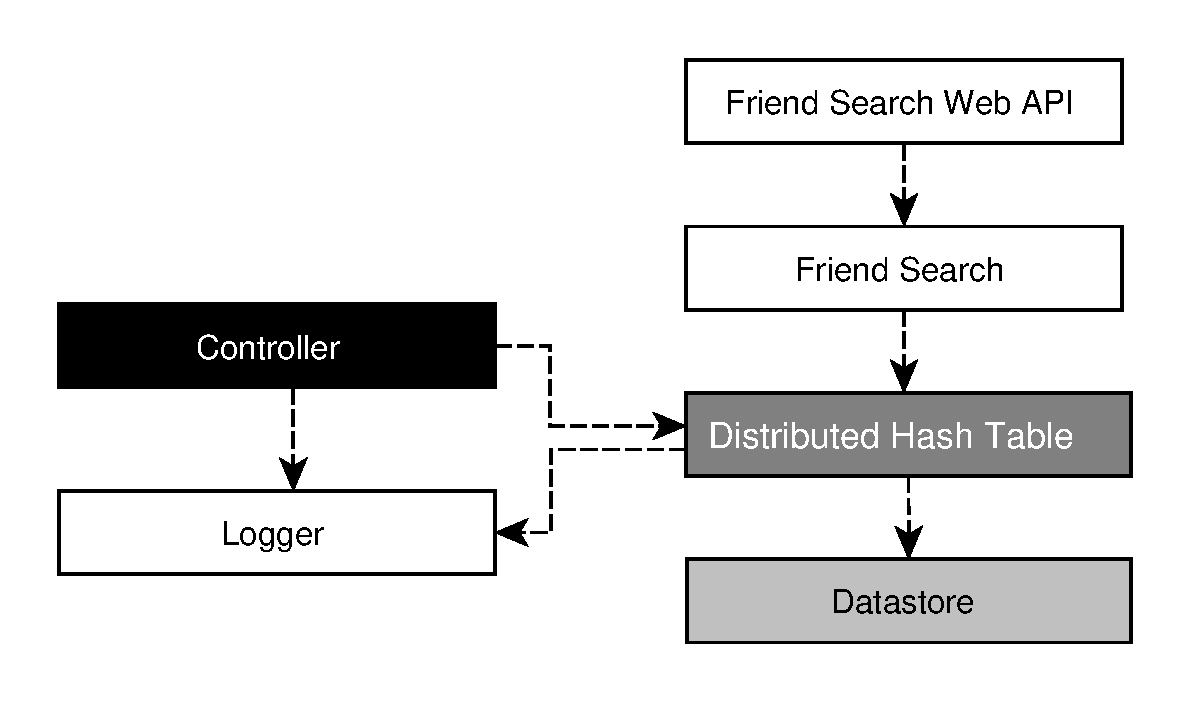
\includegraphics[width=0.9\linewidth]{illustrations/ComponentOverview.eps}
\caption{High level overview of the components of the search application. The arrows show the part a component relies on.}
\label{figComponents}
\end{center}
\end{figure}

The arrows in figure \ref{figComponents} show which components a component relies on to provide services for it. The Friend Search Web API exposes the HTTP API to the world and in turn uses the Friend Search server for resolving search queries into link records and then profile records that can be displayed to the end user. The Friend Search server uses the Distributed Hash Tables for finding the records, and the Distributed Hash Tables have local data stores that store the data items the particular Distributed Hash Table nodes are responsible for.

The controller is the component that interacts directly with the central control hub and starts and stops Distributed Hash Table nodes. It also regulates if Pastry or Chord nodes should be run.

During experimental runs, the controller is also the component that issues requests to the locally run Distributed Hash Tables.

The logger is used for logging events during experiments, and is specific to the experimental setup. While a logger would certainly be included in the final release of my search engine, the one currently implemented would not be.

\subsection{Third party code}
% Which components are not developed by me?
The Friend Search Web API in figure \ref{figComponents} uses an Erlang library called Webmachine for correctly handling HTTP requests. Webmachine in turn relies on another Erlang library called Mochiweb which the Friend Search Web API also uses in order to serialize the search results into JSON for consumption by the clients.

\section{Distributed Hash Tables}
Distributed Hash Tables are nothing but key-value stores where the data is stored across an array of machines --- yet I am implementing two of them. The reason is that Chord and Pastry differ quite significantly in the way they approach finding out on which nodes data-items are stored. Not only do they differ in the way they organize and store their routing information, but unlike Chord, Pastry uses a proximity heuristic to favour nodes geographically closer to itself when routing. These differences in routing directly translate into differences in performance as we will see in the evaluation chapter.

Specific for my implementations is that I used a bag approach where I allow multiple items to be stored under the same key. This is necessary to avoid link records with common keys replacing each other.

The Chord key-space is an integer key-space ranging from 0 up to $2^{160} - 1$. It wraps around at the end such that $2^{160} - 1$ immediately precedes 0. It can be useful to think of the key-space as circular. Just like the Chord key-space the Pastry key-space is also an integer key-space. While the Pastry paper \cite{pastry} suggests using keys in the range of 0 up to $2^{128} - 1$, I decided to let the Pastry key-space range from 0 to $2^{160} - 1$ just like for Chord, to increase code reuse between my Chord and Pastry implementations.
I assume the Pastry paper suggests using a 128-bit key space since they are easier to store efficiently in memory on 64-bit machines, which are the norm today, but other than that I can find no evidence in the Pastry paper \cite{pastry} indicating that the performance of the Pastry algorithm should be any worse using 160-bit rather than 128-bit keys.

All data stored in Chord and Pastry is stored under 160-bit keys. As a matter of fact the Chord and Pastry nodes themselves are also associated with keys in the same key-space as the data items. I use a hash of the machines public IP-address and the port number a given node is listening to in order to determine a Distributed Hash Table node's key.

A node's key plays a significant role in splitting up the key-space between the nodes in the Distributed Hash Table. For this reason it is important that the keys are evenly distributed in the key-space so the amount of key-space each node is responsible for is roughly the same.

A Chord node is responsible for all the keys greater than the key of the node's predecessor and smaller or equal than the node's own key. In figure \ref{figKeyspaceChord} the green node is responsible for the part of the key-space circle that is coloured green, the node coloured red for the part of the key-space coloured red, and likewise the yellow nodes for the part of the key-space that is yellow in colour.
A Pastry node on the other hand is responsible for all key-values that are numerically closer to the node's own key than to the key of the nodes on either side of it in the key-space. In figure \ref{figKeyspacePastry} you can see how the green and the red node each are responsible for half the key-space between them. Likewise the red and the yellow node are each responsible for half of the key-space between their respective key-values.

\begin{figure}[!htb]
\begin{center}
	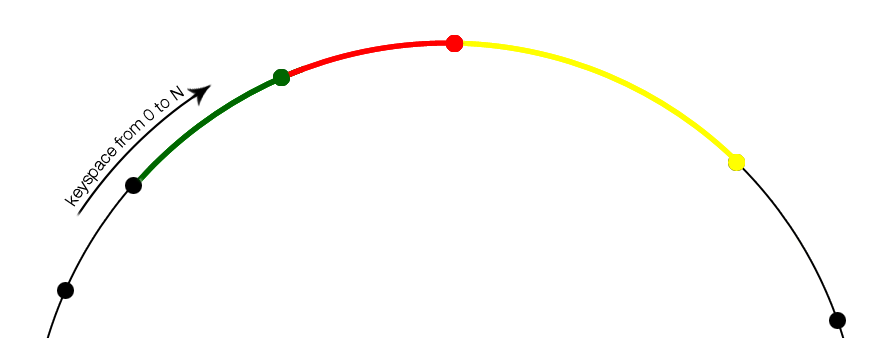
\includegraphics[width=0.9\linewidth]{illustrations/ChordKeySpace.png}
  \caption{Illustration of how the keyspace is divided between Chord nodes.}
  \label{figKeyspaceChord}
\end{center}
\end{figure}

\begin{figure}[!htb]
\begin{center}
	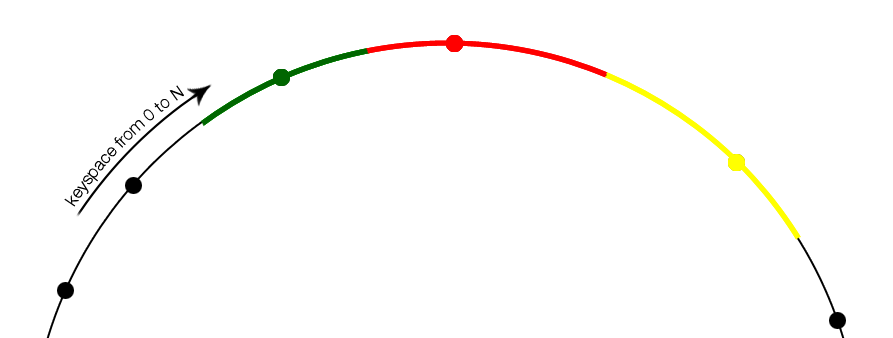
\includegraphics[width=0.9\linewidth]{illustrations/PastryKeySpace.png}
  \caption{Illustration of how the keyspace is divided between Pastry nodes.}
  \label{figKeyspacePastry}
\end{center}
\end{figure}

Just like in regular hash tables, the performance is best if a good hashing function is used to generate keys so that the keys are uniformly distributed in the key-space. This minimizes collisions but in the case of Distributed Hash Tables also ensures that the nodes in the network store roughly equal amount of data. The traffic distribution in the network depends on the distribution of the keys being requested which might not be as uniform, but if the keys requested are spread out in the key-space, the traffic, much like the data, will also be spread between the nodes in the network.

In order to be able to use Chord or Pastry interchangeably I specified a minimalistic API they should implement with functions for setting and getting values and starting and stopping Distributed Hash Table nodes.

\subsection{Data structures}
To better understand how the routing algorithms work, let us first look at the data structures used by Chord and Pastry for storing the routing information.

\subsubsection{Chord's routing table}
The Chord routing table contains an array of what in the chord jargon are called fingers.
Each finger contains a start value, depending on the fingers position in the array and the node's own id, and a reference to the first node in the Chord network with a key greater than that start value.
Additionally each finger contains an interval consisting of its own start value and the start value of the next finger.
The node stored in the $ 0^{th} $ entry of the finger array is the node's successor node, the node in the subsequent entry a node slightly further away, and the entries following after that likewise contain nodes with increasing distance in terms of the key-space from the node itself. 
The routing table stores a total of 160 entries, one for each bit in the key.

Table \ref{tableChordRoutingTable} show the Chord routing table and how each finger entry is calculated. It is taken straight out of the Chord paper \cite{chord}. The values n, m and k are the node key, number of bits used for the key and index into the finger table array respectively. 
The $ k^{th} $ finger entry has a start value half the key-space greater than the node's own key-value. The $ k-1^{th} $ entry a node quarter of the key-space further away, and so on until the nodes immediately preceding the node are found.
This construction allow nodes to quickly close in on any given key-value by contacting another node which itself is at most half the key-space away from the key-value.
In our implementation m is always 160. Please note that the array starts at 1 and not 0.

\begin{table}[h]
\caption{Values in the Chord routing table for a node with key n, using m-bit identifiers. k is an arbitrary array index into the finger array.}
\begin{center}
\begin{tabular}{ | l | l | }
  \hline                       
  Notation & Definition \\
  \hline  
  \hline  
  finger[k].start & $\left( n + 2^{k - 1} \right) mod \; 2^{m} , 1 \leq k \leq m $ \\
  \hline  
  \;.interval & $ \left[ finger[k].start, finger[k+1].start \right) $ \\
  \hline  
  \;.node & first node with key $ \geq n.finger[k].start $ \\
  \hline  
  predecessor & the previous node in the key-space \\
  \hline  
\end{tabular}
\end{center}
\label{tableChordRoutingTable}
\end{table}

In listing \ref{listingChordDataStructures} you see how I translated this into Erlang records.

\lstinputlisting[label=listingChordDataStructures,caption=Chord routing table as Erlang records]{sourceCode/chord_routing_table.erl}

\subsubsection{Pastry's routing table}
Now, how does Pastry's routing table differ from that used by Chord?
A Pastry node maintains three separate data structures: a tuple called the leaf set containing a list of the nodes preceding and a list of nodes succeeding it in the key-space, a list of nodes called the neighbourhood set that are it's neighbours in terms of the proximity heuristic used by Pastry, and a routing table. 
To make sense of the routing table let us first realize that while Chord looks at the key-space as an integer key-space in base 10, a Pastry node looks at the key-space as an integer key-space in an arbitrary base b.
The routing table is a list of lists of nodes that share increasing number of digits in the key with the node itself. The first level entry in the routing table stores a list of nodes whose keys share no digits with the node, the second level entry stores nodes that share the first digit, and so on up until the last level entry where nodes share all but the very last digit.
In a sparsely populated network, most of entries in the routing table will be left blank.
On the $ n^{th} $ level of the routing table, a node stores a list of nodes with keys that do not differ in any of the most significant digits up until the $ n^{th} $ key-digit.
A node will try to store nodes for all possible values of the $ n^{th} $ digit, so ideally a node that itself has an $ n^{th} $ digit of 0, will have entries for nodes with values 1 through b-1 in their $ n^{th} $ digit key positions.

The following code listing shows the Erlang version of the Pastry routing state.
The distance field on line 6 in the node record in listing \ref{listingPastryDataStructures} is the numeric distance between a particular node and the node maintaining the routing state, as returned by the proximity heuristic used for routing.

\lstinputlisting[label=listingPastryDataStructures,caption=Pastry routing table as Erlang records]{sourceCode/pastry_routing_table.erl}

\subsubsection{Example routing state}
The Chord and Pastry routing states can get quite abstract without a concrete example.
In figure \ref{figKeyspaceExample} I show a reference 8-bit key-space with nodes drawn as dots. The green dot represents the node whose routing state we will inspect. You will see that each node has two keys. The top one is the key as seen by Chord, and the bottom most key is the key as it is seen by Pastry which in this case interprets the keys as numbers in base 4.

\begin{figure}[!htb]
\begin{center}
	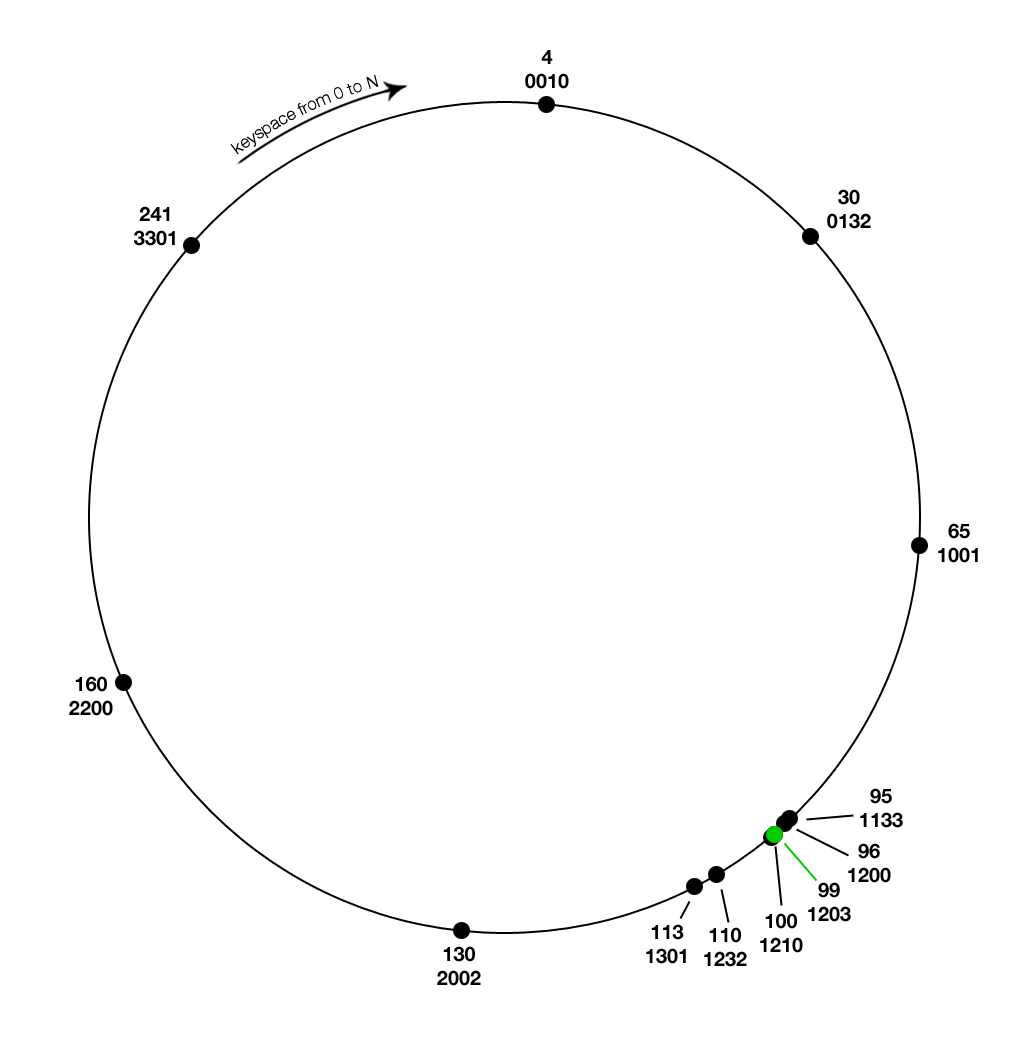
\includegraphics[width=0.9\linewidth]{illustrations/KeyspaceExample.png}
  \caption{Key-space with nodes. Each node has two keys. The top one is the key represented in base 10 as Chord sees it, and the bottom one in base 4 as seen by Pastry in this example.}
  \label{figKeyspaceExample}
\end{center}
\end{figure}

Table \ref{tableChordRoutingTable} shows the routing state held by the Chord node with key 99, while table \ref{tablePastryRoutingTable} shows the corresponding routing state for the same dot but as a Pastry node with key 1203.

\begin{table}[h]
\caption{Chord routing table for nodes in figure \ref{figKeyspaceExample}}
\begin{center}
\begin{tabular}{ | l | l | }
  \hline                       
  Field & Value \\
  \hline  
  \hline  
  % First finger
  finger[1].start & $ 99 + 2^{0} = 99 $ \\
  \hline  
  \;.interval & $ \left[ 99, 101 \right) $ \\
  \hline  
  \;.node & 100 \\
  \hline  
  % Second finger
  finger[2].start & $ 99 + 2^{1} = 101 $ \\
  \hline  
  \;.interval & $ \left[ 101, 103 \right) $ \\
  \hline  
  \;.node & 110 \\
  \hline  
  % Third finger
  finger[3].start & $ 99 + 2^{2} = 103 $ \\
  \hline  
  \;.interval & $ \left[ 103, 107 \right) $ \\
  \hline  
  \;.node & 110 \\
  \hline  
  % Fourth finger
  finger[4].start & $ 99 + 2^{3} = 107 $ \\
  \hline  
  \;.interval & $ \left[ 107, 115 \right) $ \\
  \hline  
  \;.node & 110 \\
  \hline  
  % Fifth finger
  finger[5].start & $ 99 + 2^{4} = 115 $ \\
  \hline  
  \;.interval & $ \left[ 115, 131 \right) $ \\
  \hline  
  \;.node & 130 \\
  \hline  
  % Sixth finger
  finger[6].start & $ 99 + 2^{5} = 131 $ \\
  \hline  
  \;.interval & $ \left[ 131, 163 \right) $ \\
  \hline  
  \;.node & 160 \\
  \hline  
  % Seventh finger
  finger[7].start & $ 99 + 2^{6} = 163 $ \\
  \hline  
  \;.interval & $ \left[ 163, 227 \right) $ \\
  \hline  
  \;.node & 241 \\
  \hline  
  % Eighth finger
  finger[8].start & $ 99 + 2^{7} = 227 $ \\
  \hline  
  \;.interval & $ \left[ 227, 99 \right) $ \\
  \hline
  \;.node & 241 \\
  \hline  
  predecessor & 96 \\
  \hline  
\end{tabular}
\end{center}
\label{tableChordRoutingTable}
\end{table}

\begin{table}[h]
\caption{The Pastry routing state from the Pastry nodes in figure \ref{figKeyspaceExample}. The bold digits in the routing table indicate at which digit the node keys differ from the node's own key.}
\begin{center}
\begin{tabular}{ | l | l | l | }
  \hline
  \multicolumn{3}{|c|}{Leaf set} \\ 
  \hline
  \hline                       
  Greater: & 1210 & 1232 \\
  \hline                       
  Smaller: & 1200 & 1133 \\
  \hline                       
\end{tabular}
\begin{tabular}{ | l | l | l | l | }
  \hline                       
  \multicolumn{4}{|c|}{Neighbourhood set} \\ 
  \hline
  \hline                       
  0010 & 1301 & 3301 & 1001 \\
  \hline                       
\end{tabular}
\begin{tabular}{ | l | l | l | l | }
  \hline                       
  \multicolumn{4}{|c|}{Routing table} \\ 
  \hline
  \hline                       
  \cellcolor{green} none & \textbf{0}010 & \textbf{2}200 & \textbf{3}301 \\
  \hline                       
  \cellcolor{green} 1st & 1\textbf{0}01 & 1\textbf{1}33 & 1\textbf{3}01 \\
  \hline                       
  \cellcolor{green} 2nd & 12\textbf{1}0 & 12\textbf{3}2 & \\
  \hline                       
  \cellcolor{green} 3rd & 120\textbf{0} & & \\
  \hline                       
\end{tabular}
\end{center}
\label{tablePastryRoutingTable}
\end{table}

\subsection{Routing}
%   What is different between Chord and Pastry?
%   How is routing done?
The routing algorithms for both Chord and Pastry are reasonably compact. I will try to give an intuition for how the routing works, and then just like I did for the routing state itself, show you pseudo-code from the Chord \cite{chord} and Pastry \cite{pastry} papers, before showing you the corresponding Erlang implementations.

I have omitted supporting functions from the Erlang sample code that do not add to the understanding of the routing procedure in order to keep the source code listings short and to the point.

\subsubsection{Routing in Chord}
Let us go through what happens when a Chord node wants to get the value of a key. Let us call the node that wants the value the requester, and the node that is responsible for the key the target node. I will use figure \ref{figRoutingChord} to illustrate the procedure. In the figure the nodes with the names A, B, D and E are the nodes that directly participate in finding the target node F.
When the requester wants to get the value of a key, it start by finding the node in its own routing table with a key that most closely precedes the key it wants to get the value of. In our example this is node B. It then asks that particular node if it knows about another node more closely preceding the target key. In this case node B knows about node D which has a key closer to the target key than what B itself does. The requester, node A, repeats the same question to node D and is returned node E. When node E is asked for the closest preceding node it returns itself, and it's successor F is asked for the contents of the key.

Notice how the Chord node A, the requester, is involved in all steps of the process of looking up which node stores the value of the key. This will become important in the evaluation section where we see what happens when a node cannot be connected to.

\begin{figure}[!htb]
\begin{center}
	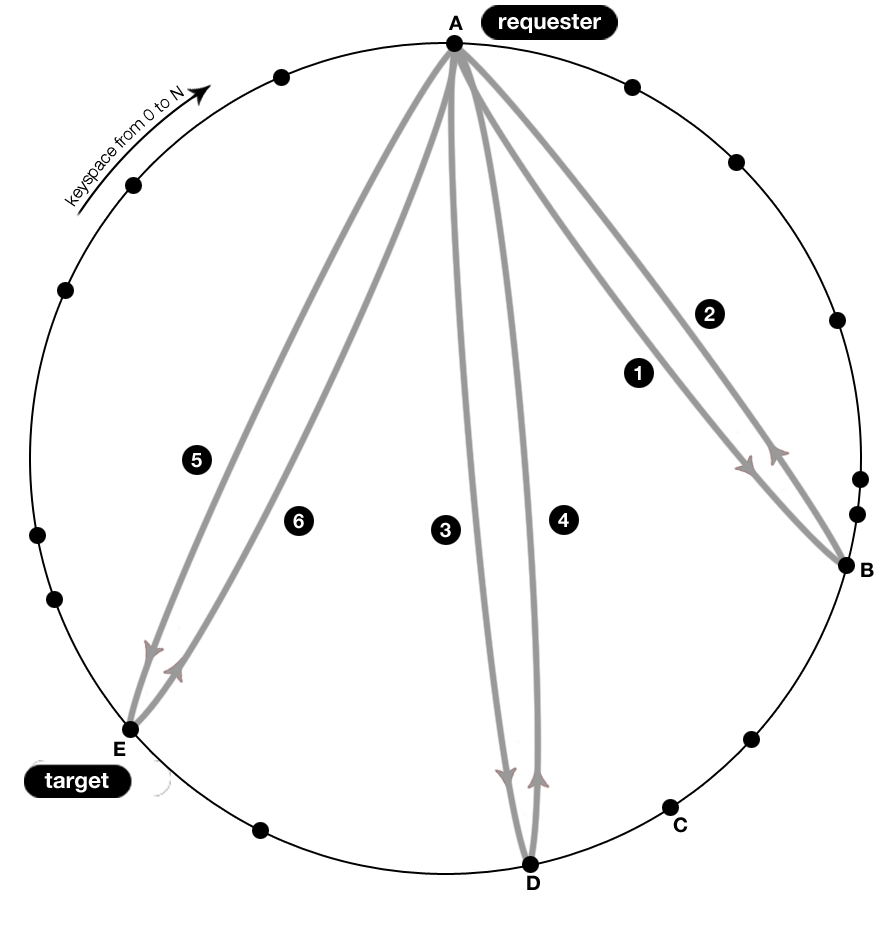
\includegraphics[width=0.9\linewidth]{illustrations/ChordRoutingSuccess.png}
  \caption{Chord's approach to routing.}
  \label{figRoutingChord}
\end{center}
\end{figure}

In the following code listings I will use the following conventions:
The syntax \verb=n.method_name()= indicates that the method with name \verb=method_name= is executed \emph{on} node \verb=n=. So when \verb=n'.method_name= is called on node \verb=n=, a remote procedure call to node \verb=n'= is being made.

Code listing \ref{listingChordPseudocode} shows the routing algorithm used by Chord as pseudo code. On line 10 in the code listing we see the method \verb=closest_preceding_finger= being invoked on node \verb=n'=. Using the routing example in figure \ref{figRoutingChord} \verb=n'= starts out as A, then changes to B etc.

\lstinputlisting[label=listingChordPseudocode,caption=Chord routing pseudo code]{sourceCode/chord_pseudocode.txt}

Let us now take a quick look at each of the three methods from listing \ref{listingChordPseudocode} in turn and compare them to their Erlang equivalents.

The \verb=find_successor= method takes a key and finds its predecessor before returning the predecessors successor.
Listing \ref{listingFindSuccessor} shows my Erlang implementation.
We see there is a very clear correspondence with the pseudo code implementation. First the predecessor node is found on line 7 and it's successor then returned on line 9.
What complicates the Erlang code slightly is that I wanted to implement the \verb=find_predecessor= while loop using recursion. I therefore had to move the assignment on line 8 in the Chord pseudo code out to the \verb=find_successor= function.

\lstinputlisting[label=listingFindSuccessor,caption=Finding the successor of a key]{sourceCode/find_successor.erl}

In code listing \ref{listingFindPredecessor} I show the Erlang equivalent of the Chord \verb=find_predecessor= pseudo code. 
In the pseudo code there are two remote procedure calls being done. One to get a node's successor, and only conditionally one requesting the node's closest preceding finger.
In my implementation these two remote procedure calls have been made into one and for this reason this call has been moved to the very front of the function.
Notice how on line 11 in the Erlang implementation we use recursion rather than the while loop used in the pseudo code. The equivalent of line 8 in the Chord pseudo code had to be moved out to the \verb=find_successor= function.

\lstinputlisting[label=listingFindPredecessor,caption=Finding the predecessor of a key]{sourceCode/find_predecessor.erl}

The procedure for finding the \verb=closest_preceding_finger= follows below. Unfortunately it is slightly more complicated than the pseudo code equivalent. Since I for fault tolerance am storing a list of successors rather than a single successor, the case of the $ 0^{th} $ finger entry has to be handled separately. 
I factored out the bounds checking done at line 16 in the Chord pseudo code into a helper function called \verb=check_closest_preceding_finger= to avoid having to duplicate it in the \verb=closest_preceding_finger= function.
This function in turn makes a call back to \verb=closest_preceding_finger= if the finger entry is not a match.
The function in listing \ref{listingClosestPrecedingFinger} recursively looks at each finger in the routing table, checking if it is valid and returning the first one it finds that is.

\lstinputlisting[label=listingClosestPrecedingFinger,caption=Returns the node most closely preceding the key]{sourceCode/closest_preceding_finger.erl}

The bounds check is implemented in the helper function \verb=check_closest_preceding_finger= in listing \ref{listingCheckClosestPrecedingFinger}.

\lstinputlisting[label=listingCheckClosestPrecedingFinger,caption=Check if a finger is the closest known finger to a key. Returns the node most closely preceding the key]{sourceCode/check_closest_preceding_finger.erl}

\subsubsection{Routing in Pastry}
The Pastry approach differs quite significantly from Chord's approach to routing.
The most significant difference is that while a Chord node actively looks for the node responsible for a key, and when that node has been found contacts it to have it perform whatever task needs doing, Pastry instead performs message passing, where the message itself can contain information about whatever task the node wants done.
Also just like when sending mail through the postal system, the node loses visibility of the messages progress as soon as it has been sent. This has the benefit of reducing the communication overhead and giving the sender time to perform other tasks or aid other nodes in their message sending while making it harder to notice if a message get lost.

I illustrate the process in figure \ref{figRoutingPastry} where the requester of a key-value, node A, sends a \emph{lookup message} to the key it wants to look up. First node A checks its own routing state for the node it knows about with a key closer to the target key than its own and sends its message to it. In this case this node is node B. B in turn does the same and forwards the message to node D which in turn sends it on to the target node F. In the final step node F contacts the requester, node A, to let it know it is the node responsible for the value of the requested key. 

\begin{figure}[!htb]
\begin{center}
	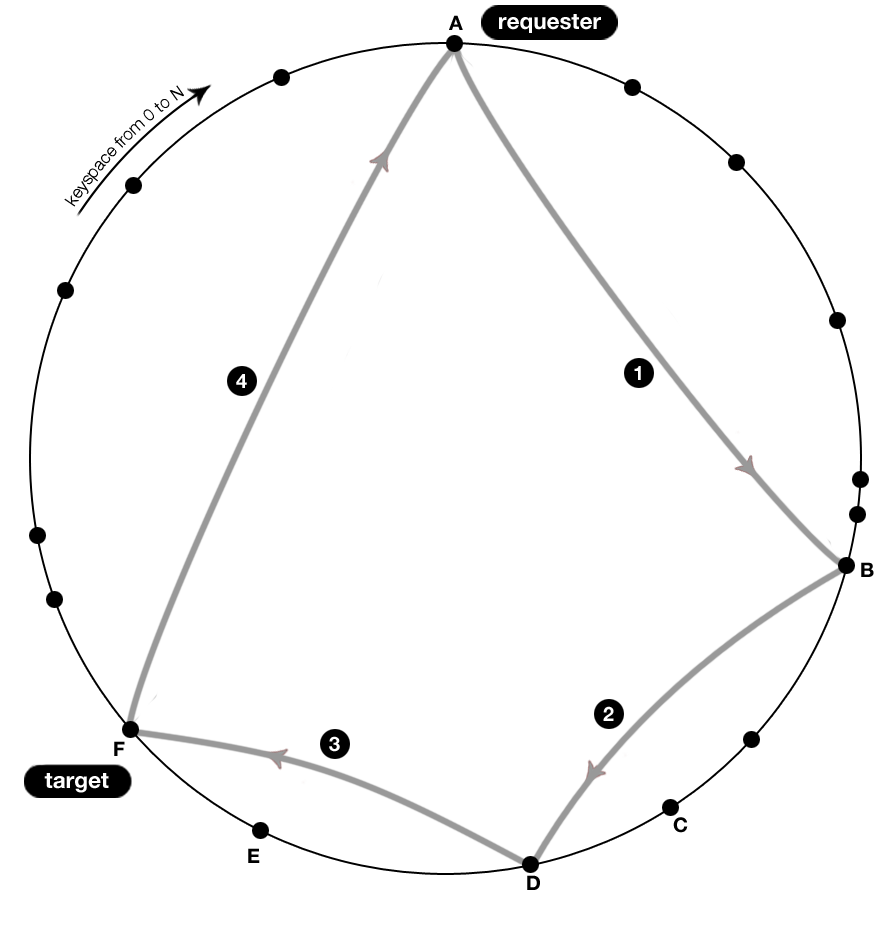
\includegraphics[width=0.9\linewidth]{illustrations/PastryRoutingSuccess.png}
  \caption{Pastry's approach to routing.}
  \label{figRoutingPastry}
\end{center}
\end{figure}

The following Pastry routing pseudo code is a slightly adapted version of the pseudo code presented in the Pastry paper \cite{pastry}.
It shows the method for routing a message for a target key k at a node with key n.

The Pastry routing approach works as follows: The node that is about to forward the message first checks if the recipient is in its leaf set. If it is it delivers the message directly. The recipient could also be itself.
If there is no match in the leaf set, the routing table is used to find a node that shares an additional digit with the key with the message key compared to the node performing the routing. If there is no match in the routing table either, the Pastry node falls back to forwarding the message to any node it knows about that has a key numerically closer to the message key than the key the node itself has.

\lstinputlisting[label=listingPastryPseudocode,caption=Message routing pseudo code for Pastry]{sourceCode/pastry_pseudocode.txt}

My Erlang implementation, rather than being a direct translation of the pseudo code, takes the essence of what the Pastry routing algorithm tries to accomplish, and implements that.

The code in listing \ref{listingRouteMsg} shows my main Erlang \verb=route_msg= function. 
Just like the pseudo code n listing \ref{listingPastryPseudocode} it tries routing via the leaf set, then the routing table and if all else fails to any node that is closer to the target key.

\lstinputlisting[label=listingRouteMsg,caption=Routes a message towards a recipient]{sourceCode/route_msg.erl}

In listing \ref{listingRouteToLeafSet} we see that if the match in the leaf set is the node itself, then on line 5 the message is delivered to the main pastry application. Otherwise the message is forwarded to a closer node if appropriate on line 7.

\lstinputlisting[label=listingRouteToLeafSet,caption=Routes a message to the leaf set if applicable]{sourceCode/route_to_leaf_set.erl}

If routing to the leaf set fails (line 3 in listing \ref{listingRouteToLeafSet}), the node tries routing the message to a node in the routing table sharing more digits in the key with the message key than what itself does. Again, just like when routing to the leaf set, if the best match is itself, the message is delivered. This function is shown in code listing \ref{listingRouteToNodeInRoutingTable}.

It is not quite as easy to see how this code listing corresponds to the pseudo code. For example, in listing \ref{listingPastryPseudocode} there is nothing that directly correspond to getting the length of the shared key path as we see on line 9 in the Pastry pseudo code in listing \ref{listingPastryPseudocode}. Instead what the Erlang implementation does is find all the nodes in the routing table that share as many key digits with the message key as the node itself does (line 2) in addition to the \verb=PreferredKeyMatch= (also line 2) which is the shared key-segment plus the first digit in the message key that differs from the key of the node itself.
On line 4 we look for a node in the list of nodes which shares all the digits in the \verb=PreferredKeyMatch=. If there is one then the message is passed on to that node and if there is none, we return empty handed.

\lstinputlisting[label=listingRouteToNodeInRoutingTable,caption=Routes a message to a node in the routing table]{sourceCode/route_to_node_in_routing_table.erl}

If all other routing approaches fail, the last resort the Pastry node has is to find any node that is numerically closer to the key than what itself is. Code listing \ref{listingRouteToCloserNode} shows the Erlang implementation finding the key segment shared between the message key and the node's key (line 2) and then finding all the nodes it knows about that share this key segment (line 3). On line 7 the node numerically closest to the message key is found and the message either forwarded or delivered.

\lstinputlisting[label=listingRouteToCloserNode,caption=Routes a message to any closer node]{sourceCode/route_to_closer_node.erl}

\subsection{Replication of data}
My implementations of Chord and Pastry both replicate data amongst their immediate neighbours for fault tolerance. While replication was only proposed as an extension in the Chord \cite{chord} and Pastry \cite{pastry} papers, I thought it worthwhile adding this functionality since my intended use case was a search engine where I did not want data to become unavailable if an online social network provider decided to stop using my search network.

\section{Search server}
% Search server
The search server is what glues together the client facing HTTP API and the Distributed Hash Tables. It receives the search queries from the clients, converts them into appropriate keys that it can lookup in the Distributed Hash Tables, and resolves link records it gets returned to full profile records that can be shown as search results.

The current implementation is rather na\"ive, and while it does basic ranking of results, prioritising what it predicts are better matches, it performs no caching of results which would significantly improve the performance.

\section{Central control hub}
% Hub control server
% Focus on testing and evaluation
The central control hub is an application that runs under a domain name known by all application instances of my search engine.
When the search engine application is started on a machine, it registers itself with the control hub which in turn tells it what Distributed Hash Table should be used and how many nodes and of what Distributed Hash Table type should be run.

When new Distributed Hash Table nodes are started they also contact the control hub to get information about which other nodes they should try to connect to in order to join the Distributed Hash Table network.

The control hub is the only single point of failure in the system. If it becomes unavailable, no new search engine hosts can join because they cannot register and get information about which Distributed Hash Table type is being used, nor can the existing hosts start new Distributed Hash Table nodes because the nodes cannot contact the central control hub to get information about nodes they could use to join the Distributed Hash Table network. All hosts that are already registered remain active, and once a Distributed Hash Table node has started it runs fully independently of the central control hub application.
One could allow hosts to start new nodes by directly telling them about other known hosts they can connect to, but that functionality is currently not implemented.

The experiments used to evaluate the system are also initiated by the central control hub through a web interface (figure \ref{figHubApp}) that allows me to set the rate at which requests should be issued and the duration of the experiment. The requests themselves are issued individually by each host running the Distributed Hash Table nodes.

\begin{figure}[!htb]
\begin{center}
	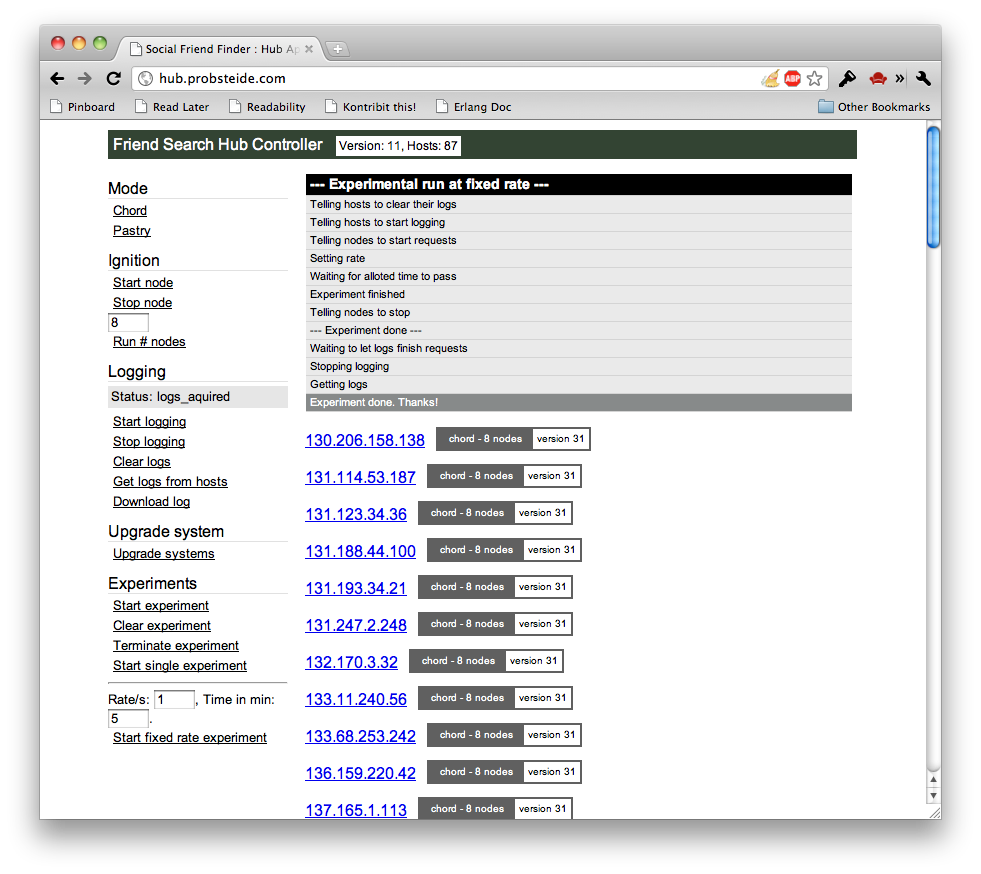
\includegraphics[width=0.9\linewidth]{illustrations/HubApp.png}
\caption{The Hub Application interface running on the central control hub. Shown here is the web interface that allows me to start and stop nodes, change between using Chord and Pastry, and start and stop experiments}
\label{figHubApp}
\end{center}
\end{figure}

Initially fully automated experiments were supported as outlined in my project briefing, but later, while evaluating my system, I removed the feature as it was impractical and didn't give me enough flexibility to run the experiments I needed.

\section{Supervision for fault tolerance}
One of Erlang's main strengths is process supervision.
The supervision behaviour which is a part of the standard library makes it trivial to write processes supervising others. These processes are responsible for the lifetime behaviour of the processes they supervise, starting them when needed, restarting them if they terminate prematurely and stopping them when the application terminates. All supervisors with the exception of the root supervisor are themselves also supervised.

Process supervision is an important feature as it encourages designing minimal and isolated modules with individual life cycle control that can fail independently without bringing down the system. As failing modules are automatically restarted without impact on other components, one can easily build systems with high availability.
Another direct benefit also encouraged by Erlang and it's designers is to write optimistic code handling what you as a designer think of as the optimal case, rather than practising defensive coding where you constantly have to check for malformed inputs. This is possible as malformed input which would cause a process to crash does not affect the systems availability since the crashed process is automatically and immediately restarted. The direct benefit of this approach is that the code base becomes smaller and much easier to read and maintain.

Figure \ref{figSupervisionTree} shows the supervisors and the servers used in the main friend search application I developed.

\begin{figure}[!htb]
\begin{center}
	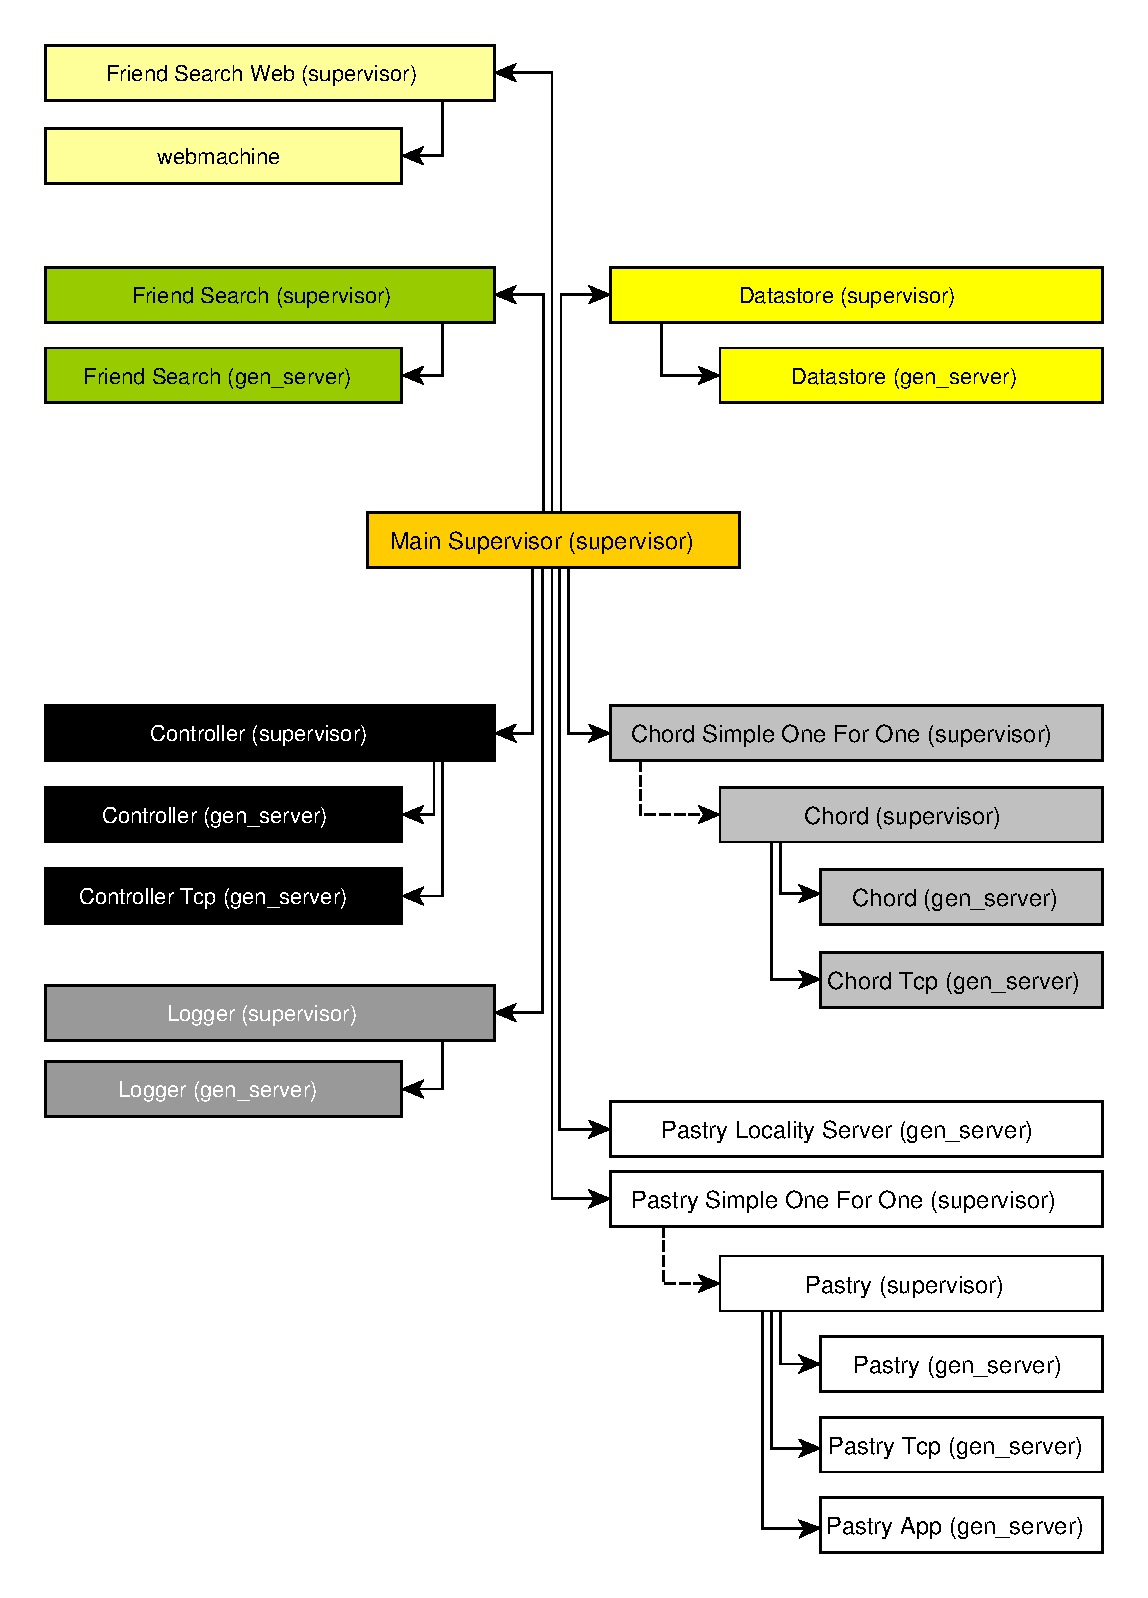
\includegraphics[width=0.9\linewidth]{illustrations/ClientSupervisionTree.eps}
  \caption{This figure shows the hierarchy of supervisors and the servers they supervise.}
  \label{figSupervisionTree}
\end{center}
\end{figure}

The root supervisor, represented by the box in the middle of figure \ref{figSupervisionTree}, supervises a wide range of other supervisors, all of which, with the exception of the Distributed Hash Table supervisors, supervise servers that are started at the same time as the application. 
The Chord and Pastry supervisors are a special kind of supervisor. They do not initially start any children, but can be signalled to start and maintain an arbitrary amount of children. This feature allows my system to at runtime dynamically adjust the number of Distributed Hash Table nodes that are run.


\section{Hot code reloading}
The Erlang virtual machine supports hot code reloading.
I built a code distribution service on top of this functionality, that automatically updates the binary code of all running nodes whenever I pushed code changes to my code repository.

This greatly reduced the time it took to change small bugs and experiment with changes after I had deployed my code to a large network of machines.

\mbox{}

In this chapter we have looked at how I developed my system. We looked at high level components and went into details of how routing differs between Chord and Pastry. We then looked at the other central components of my project, the central controlling hub and the search server.
Finally we had a brief look at Erlang's supervisors and hot code reloading.

% * How many of original goals were achieved? Proved to have been achieved
% * Did the program really work?
% *! Credit for interesting conclusion

% ************
% Should have: 
% 	intro
% 	content
% 	summary
% ************
\section{Evaluation}
\subsection{Experimental design}
In this section, \textit{host} refers to a physical machine, while a \textit{node} is an instance of a distributed hash table running on a host. Each host will run one or more nodes.

The focus will be on testing the practicality of using the distributed hash tables as back end stores for my friend search engine, and mainly focus on different aspects of resource consumption.

\paragraph{What will be tested}
Four experiments will be performed: 

\begin{enumerate}
\item The time it takes to perform a lookup
\item The number of nodes involved in a lookup
\item The amount of bandwidth required to do a lookup
\item The amount of bandwidth required to maintain routing state
\end{enumerate}

Each experiment will be performed separatly for chord and pastry, in each case for networks of different sizes.

The experiments will follow a factorial design where the factors are:
\begin{itemize}
\item The number of nodes in the network
\item The rate of requests
\end{itemize}

In each experiment, given N hosts, the number of nodes will be 2$^{k}$N --- k taking levels 0 through 3 per experimental run. As the number of nodes involved in any lookup is thought to be proportional to the logarithm of the number of nodes in a network, this seems likely to give interesting data to analyse.

None of these experiments rely on querying for real data. Keys to lookup will therefore be generated by hashing a combination of a counter value and the identity of the host performing the request. This is likely to give an even spread of keys.

\subparagraph{The time it takes to perform a lookup}
This is an interesting experiment in terms of the expected end-user experience. We want to observe how the response time is affected by network size and request rate. The outcome of this experiment dictates how complicated queries the network can sustain, and more concretely if predictive searches in its current form can be sustained on a larger scale. Each host will individually issue request to produce a balanced load.

The factors are network size and the rate of requests. 
For each level of network size, each host will issue requests serially at increasing levels of parallelism until any one host sees a failure rate of more than 25\%. Each level of parallelism will be kept for a minute.

The number of runs required for this experiment depends on how well the networks cope under load.

\subparagraph{Number of nodes involved in a lookup}
This experiment focuses on what fraction of the network has to be involved in a request and how this scales with the size of the network. This is relevant as the number of nodes involved can indicate how well the network will manage under heavier load.
The request rate is irrelevant for this experiment -- the only factor is network size, and the response variable the number of nodes involved in a lookup.

For one run of this experiment, we need data for each of the 4 possible levels of network size.

\subparagraph{The amount of bandwidth required to do a lookup}
This experiment is interesting in terms of real world applicability. The nodes are likely to be hosted by end users paying for the bandwidth consumed by their servers. The actual bandwidth consumption will to a certain extent be implementation specific, but the experiment will give us an indication of how chord and pastry compare.

This experiment will be performed as part of the experiment counting the number of nodes involved in a lookup.

\subparagraph{The amount of bandwidth required to maintain routing state}
This experiment also helps determine if the implementations are usable in a real world setting.
The bandwidth consumption will depend on the configurable options of chord and pastry. This makes a fair comparison hard. Configuration values will chosen that generally prove to give good \textit{routing} performance.

This experiment will measure the bandwidth consumed per node over a 5 minute window per network size.

\paragraph{What will not be tested}
The behaviour of the networks depends on their different configurable options. 
In chord you can adjust the number of successors it keeps in touch with, and the frequency at which these relations and the routing table is kept up to data.
In pastry in addition to choosing the rate at which the routing tables are maintained, there is a \textit{b-parameter} influencing how many routing steps will be required but also the size of the routing tables.

Since the configurable parameters do not directly correspond between the two implementations, their levels will be fixed at values that generally give good and consistent \textit{routing} performance.

While both my implementation of chord and pastry replicate their data for fault tolerance, this behaviour will not be tested. It is expected that the network size will not fluctuate wildly over time in a real world deployment, as the nodes are likely to be hosted on servers in operation over long periods of time. This is very much unlike other distributed hash table usage scenarios, like file sharing, where the amount of nodes joining and leaving the network at any given time can be significant (I don't have any data to back this claim with, but it sounds reasonable!?).


\subsection{Experimental results}

% Conclusion (?)
% 	Make it clear in first paragraph what your project was
% 		about and how well you've done it
% 	Will fill in marking sheet after they have done it.
% 	Remind them how awesome project is
% 	If did again, might do... XYZ
% * Refer back to Introduction.
% * How would have planned the project if starting again with benefit of hindsight

% ************
% Should have: 
% 	intro
% 	content
% 	summary
% ************

\section{Conclusion}

\chapter{Acknowledgements}
I want to thank Dr David Evans for supervising my project and for always being supportive and willing to help and give tips when I got stuck.

I want to thank Felix Bauer for spending countless hours helping me make sense of my experimental results and helping me out with \LaTeX.

I want to thank Eugene Chan for providing general moral support.

I want to thank Dr David Eyers for all the help he gave me while I was planning my project and also for giving feedback on the project proposal.

And finally I want to thank Dr Robert Harle and Prof Jon Crowcroft for taking the time to read through drafts of my dissertation.

\section{}


\appendix
\addtocontents{toc}{\protect\contentsline{chapter} {Appendix}{}}
\section{}


\cleardoublepage
\chapter{Project Proposal}

% Draft #1 (final?)

\vfil

\centerline{\Large Friend search for distributed social networks }
\vspace{0.4in}
\centerline{\large Sebastian Probst Eide, St Edmunds College }
\vspace{0.3in}
\centerline{\large Originator: Sebastian Probst Eide}
\vspace{0.3in}
\centerline{\large 4 October 2010}

\vfil

\subsection*{Special Resources Required}
Personal laptop for development and initial testing (1.86 Ghz, 2GB Ram) \\
CL machine with the Erlang VM installed as a backup \\
Virtual Server infrastructure, the like of Amazon EC2, for parts of the evaluation \\
\vspace{0.2in}

\noindent
{\bf Project Supervisors:} Dr David Eyers and Dr David Evans
\vspace{0.2in}

\noindent
{\bf Director of Studies:} Dr Robert Harle
\vspace{0.2in}
\noindent
 
\noindent
{\bf Project Overseers:} Unknown ********** PLEASE UPDATE! ***********

\vfil
\pagebreak

% Main document

\section*{Introduction}

It is hard to get started using independent, distributed online social networks as it is frequently difficult to find and connect with your existing friends, not knowing in which social networking system(s) they host their profiles and where those networks are hosted. The purpose of this project is to lay the foundation for a decentralised and distributed friend search engine that can be offered alongside installations of independent social networks allowing users to easily reconstruct their social graph in the online social network(s) of their choice. The focus of the project will be on the data storage layer of the search engine. I will compare and contrast different Distributed Hash Tables that I implement in Erlang. Erlang is chosen because it is known to be well suited for developing concurrent and distributed systems.

A front end, allowing basic searches to be performed, will also be created, but mainly to provide a way to rapidly exercise the data storage layer. More user-oriented functionality needed to allow the project to be used on a larger scale will be left out so as to limit the scope of the project.

\section*{Work that has to be done}

There are a number of distributed hash table designs available.\footnote{ Wikipedia currently lists 8 different protocols } I have decided to implement and compare the following three, chosen because they are well documented algorithms but importantly differ in the way they perform their routing: Chord, Kademilia and Pastry. As an example in how they differ, consider how Pastry allows for heuristics based on anything from ping to available bandwidth or combinations thereof, Kademilia uses XOR arithmetic to determine the distance between nodes as a routing heuristic, while Chord has none of the above, using simplicity as its strength. These different approaches to the same problem make the algorithms excellent candidates to compare.

The main parts of the project are to:

\begin{itemize}
  \item Implement the data storage layer of the search engine in Chord, Kademilia and Pastry using a uniform API that allows the system to use any one of the three without additional changes
  
  \item Implement infrastructure that facilitates testing and monitoring of the system. More specifically it should allow:

  \begin{itemize}
    \item Starting and stopping virtual servers across the different service providers to minimize server rental costs between testing sessions. The servers will be used to test different aspects of the distributed hash tables
    \item Start and stop search nodes across the physical servers
    \item Display how many search nodes are available in the system, and potentially some metric for how they are interconnected in terms of latency and bandwidth
    \item Add and remove test data from the system. The system will be tested with \emph{Database of names} from Facebook which I have access to. It is of significant size and importantly, contain keys with non-random distributions making for a more realistic dataset
    \item Perform repeatable load testing on the system where tests as an example could compare read/write performance for different key and value sizes and different numbers of key-value pairs
    \item Count the number of jumps and the time a key lookup needs in order to find a data item, in addition other appropriate descriptive statistical measures for writes and lookups in fixed key-value datasets
    \item Being able to eliminate and add subsets of storage nodes in a repeatable fashion to test how the different Distributed Hash Tables cope with nodes disappearing and appearing
  \end{itemize}

  \item Setup a Linux image that can be run across Infrastructure as a Service providers\footnote{Vagrant seems like a likely candidate to help automate this (http://vagrantup.com)}

  \item Implement a web front end to allow users to perform basic searches across the data storage layer

\end{itemize}

Please note that while the following aspects of the search server are secondary to the project and will not initially be implemented, they all, should time permit, serve as excellent project extensions:

\begin{itemize}
  \item Fuzzy searches allowing the user to misspell names. 
  \item Support composite keys to allow searching for different attributes of a record
  \item Predictive searches
  \item Searches taking knowledge about social circles from online social networks, or similar metadata, into account in order to more intelligently prioritise and order the search results returned to the user
  \item Protections against malicious use of the storage network like broadcasting data, attempting to overload nodes with requests or using the network to store spam or pollute the namespace with spammy records
\end{itemize}


\section*{Starting Point}

I have a reasonable working knowledge of Erlang and Linux and development of web based systems. The algorithms that will be implemented have all previously been implemented in other languages, and are used in production systems, so finding information about them should be possible. I have not yet used Amazon EC2 or any of the other Infrastructure as a Service (IaaS) providers that could be used to perform testing on the system in a distributed manner.


\section*{Success criterion}

I regard the project as successful if I have working implementations of the three Distributed Hash Tables that allow me to set and retrieve values based on keys across a distributed network of machines, and also metrics for how the performance of key-lookup varies by node-, key-count and distributed hash table type and recommendations for future work based on the metrics collected.

The search component of the project, which is the application part that uses the distributed hash tables as a datastore to allow users to find their friends, has been left out of the success criterion due to it being harder to quantify and evaluate well.

\section*{Difficulties to Overcome}

The following main learning tasks will have to be undertaken before 
the project can be started:

\begin{itemize}

\item To learn and fully understand the Chord, Kademilia and Pastry algorithms.

\item To learn how to do network communication in Erlang other than the built in message passing. I prefer the individual nodes to communicate over TCP or UDP as that frees the design from assumptions regarding the language of implementation, and also removes the substantial overhead incurred by having each Erlang VM keep track of the state and availability of all the other nodes network wide, which would be in stark contrast with the distributed hash tables need to only maintain rather minimalistic routing tables. Additionally there are security issues when allowing Erlang VMs to connect directly in untrusted networks as any node is allowed to execute arbitrary code on any other connected node

\item To find a way to test the system on geographically distributed nodes.

\end{itemize}


\section*{Resources}

Some aspects of this project (amongst others the heuristics in Pastry that take locality into account when routing) are more interesting to test in nodes that are geographically distributed. For this reason using server instances from a provider like Amazon AWS or PlanetLab seem like a good idea. Ways of getting access to time on such infrastructure for academic purposes is currently being looked into. For the majority of the development cycle local testing will be just as interesting and can be done on my development machine.

This project requires no additional file space on University machines. I will be hosting the project source code and dissertation files in a repository on github.\footnote{http://github.com/sebastian/Part-2-project}
If my machine breaks down, the development can be continued on any Unix based machine that has VIM, git and the Erlang VM installed.

\section*{Work Plan}

Planned starting date is 15/10/2010. 

Below follows a list of tasks that need to be done:

\begin{itemize}
  \item Work through the theory behind Chord, Kademilia and Pastry and other items listed under \emph{difficulties to overcome} (2 weeks).
  \item Implement initial version of Chord, Kademilia and Pastry in Erlang (4 weeks)
  \item Implement test harness to perform testing of the system (4 weeks)
  \item Implement a web frontend for search alongside a search server written in Erlang, that uses the distributed data storage layer for its data (2 weeks).
  \item Write dissertation (6 weeks).
\end{itemize}

\subsection*{Michaelmas Term} 

By the end of this term I intend to have completed the research and learning tasks and have finished the first implementations of the Distributed Hash Tables in Erlang. In the vacation that follows I intend to make a good start on the testing harness and do a little work on the search server.


\subsection*{Lent Term}

In the first half of this term I intend to finish the test harness and search server and spend time testing the system and solving problems. The tests could follow a factorial design where distributed hash table type, number of nodes, key-size, payload size, number of entries in the system and geographical distribution are all factors worth considering. What levels should be considered for each factor is yet to be determined and will become clearer as the project develops.

In the second half of this term I tend to get an initial draft of my dissertation written.


\subsection*{Easter Term}

In this term I plan to polish the dissertation. The estimated completion date is the 15th of May, leaving a couple of days to let the dissertation rest before giving it a final read and correcting last minute mistakes before the due date on the 20th of May.


\end{document}
